\newcommand{\sdsstriquinttable}{\newlength{\cw}
\settowidth{\cw}{\textbf{Percentage of images recognized}}
\begin{tabular}{|c|D{.}{.}{3.2}|D{.}{.}{3.2}|D{.}{.}{3.2}|}
\hline
\multicolumn{1}{|c|}{\textbf{CPU time}} &\multicolumn{3}{c|}{\textbf{Percentage of images recognized}} \\
\cline{2-4}
\multicolumn{1}{|c|}{(per image)} & \multicolumn{1}{c|}{\makebox[0.35\cw][c]{Triangles}} & \multicolumn{1}{c|}{\makebox[0.35\cw][c]{Quads}} & \multicolumn{1}{c|}{\makebox[0.35\cw][c]{Quints}} \\
\hline
\makebox[\pointonesec][r]{$0.1$ s} & 0.20  & 57.45  & 23.35 \\
\makebox[\pointonesec][r]{$1$ s} & 28.07  & 92.20  & 36.67 \\
\makebox[\pointonesec][r]{$10$ s} & 78.58  & 99.28  & 72.75 \\
\makebox[\pointonesec][r]{$100$ s} & 99.15  & 99.33  & 95.08 \\
\makebox[\pointonesec][r]{$1000$ s} & 99.97  & 99.33  & 96.25 \\
\hline
\end{tabular}
}
\newcommand{\sdsstriquintntrynmatchfig}{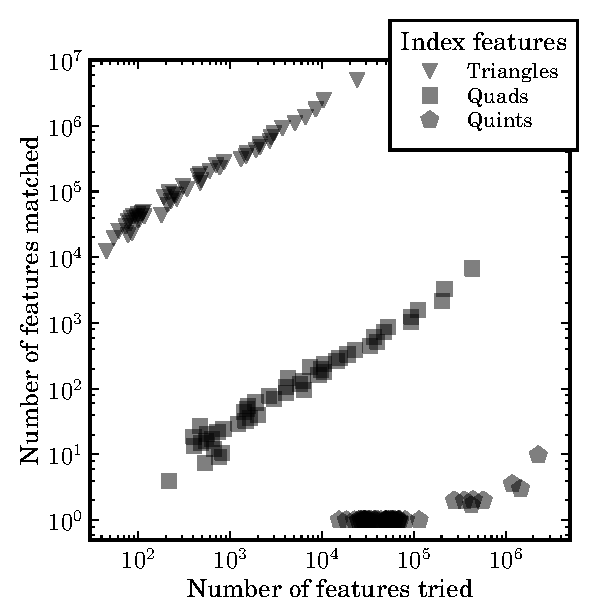
\includegraphics[width=1.000000\figunit]{sdss-triquint-ntrynmatch}}
\newcommand{\sdsstriquinttimefig}{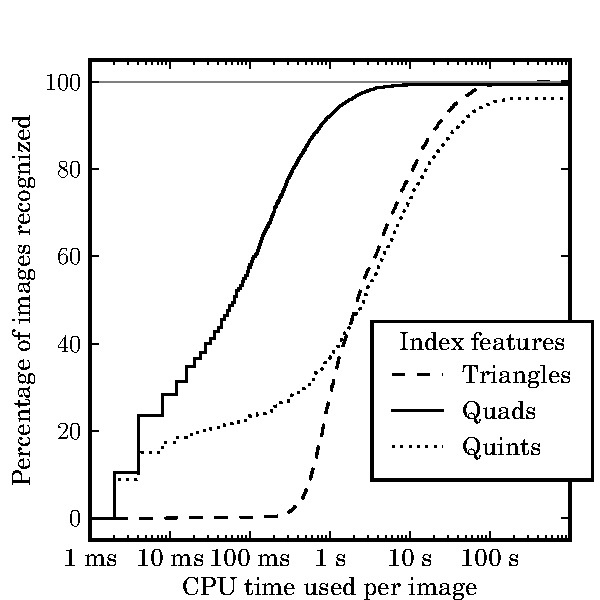
\includegraphics[width=1.000000\figunit]{sdss-triquint-time}}
